%!TEX root = mb.tex

\section{System implementation} \label{sec:impl}
\eat{
\todo{this is important to write properly because it is a systems paper and there were some nontrivial decisions}.

Things to cover:

- gateway and middlebox implementation

- explain why the firewall hardware does not change (or was that above?)

- second flow udp/tcp

- might want to explain these points made in intro: "
Sylvia, it would be great if you could read and revise the paper. Feel free to edit directly in tex!
We really need your feedback at this stage."

- new packet structure and headers -- multiple layers of headers? graph? (there is some text and a figure in a google doc about this)

- some things are specific to web proxy from what I remember
}

We now describe the MBArk architecture and implementation. 
We first describe the outsourcing and redirection implementation (\S\ref{sec:redirection}); we then describe the packet-level encoding mechanisms (\S\ref{sec:packets}).
Finally, we discuss how middleboxes are modified to enable operation over encrypted flows; we also discuss how and why some middleboxes (such as firewalls and NATs) do not require any modifications to support MBArk (\S\ref{sec:mbimpls}).

\subsection{Redirection Architecture}

\begin{figure}[t]
  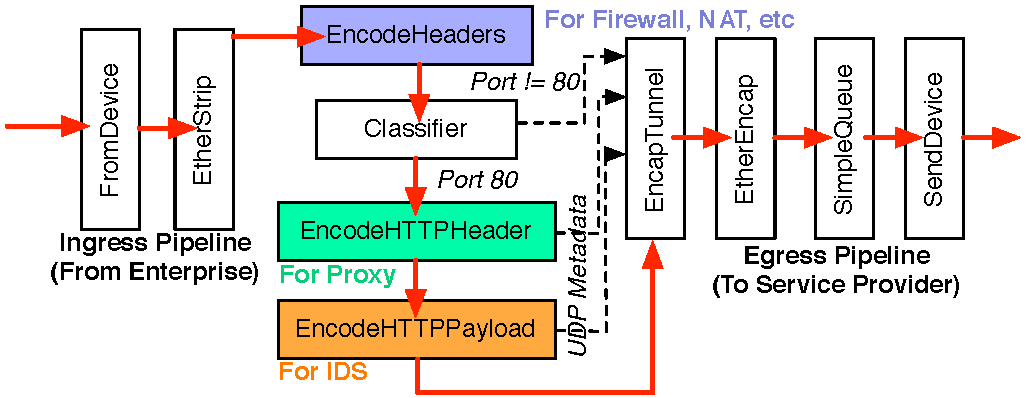
\includegraphics[width=3.25in]{fig/gatewaydiag}
  \caption[]{Gateway software architecture (enterprise to service provider).}
\end{figure}



\begin{itemize}
  \item Components: sender, receiver, gateway, cloud
  \item Sketch: redirection, follows essentially from APLOMB approach
  \item Ref to Figure 1
  \item How we built and tested:
    \begin{itemize}
      \item HW components, server specs
      \item Deployed on EC2 using Click-based implementations for all middleboxes
      \item Gateway scheme, components, discussion about Figure~\ref{fig:gateway}.
    \end{itemize}
\end{itemize}

\subsection{Packet Encoding}


\begin{itemize}
  \item Describe Figure~\ref{fig:gatewayops} -- packets come in, and are converted to encrypted v6 packets either reprsenting the packet itself of metadata for the IDS.
  \item How do we do the v4-v6 conversion? Discuss Figure~\ref{fig:packet}. Why each field is the way it is. Emphasize: this is a VALID IPv6 packet, even though the header fields are encrypted!
\end{itemize}

\subsection{Middlebox Implementations}

\begin{figure}[t]
  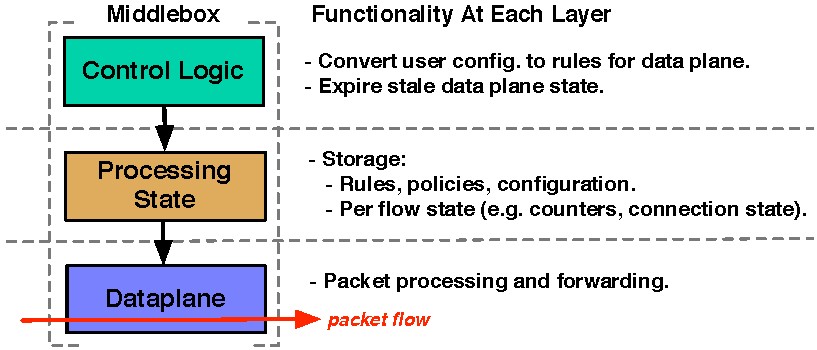
\includegraphics[width=3.25in]{fig/mbarch}
  \caption[]{Typical middlebox software architecture. To be compatible with \sys, most middleboxes only require changes in the control logic. For these devices, packet processing operations in the dataplane remain unmodified and performance-competitive.}
\end{figure}

\subsection{Unmodified Middleboxes}
\begin{itemize}
  \item IP Firewall, NAT, IP Forwarding, LB L4
  \item Operations: Match, Match/Replace, Range -- on specific fields
  \item Why no change? Packets are valid IPv6 packets, and all we need to do is have encrypted rules as well.
  \item How rules are encrypted, how often rules must be updated for Range (basically never) which we show in eval.
\end{itemize}

\subsubsection{Modified Middleboxes}
\begin{itemize}
  \item Exfiltration, IDS, Proxy, App Firewall, L7 Load Balancer
  \item Why change? All perform some kind of DPI -- variable offset, and variable operation. Key thing we need is the match, but the encoding that comes out looks very different than the normal packet.
  \item Required modifications:
    \begin{itemize}
      \item Exfiltration, IDS, App Firewall -- same as BB
      \item Proxy -- mapping from crypto to table. Note that the session termination code -- which is complicated! -- does not change at all because these are all header operations on what looks liek a valid IPv6 packet.
      \item L7 Load Balancer -- I actually don't know how this one works?
    \end{itemize}
\end{itemize}
